\begin{figure}[htbp]
  \centering
  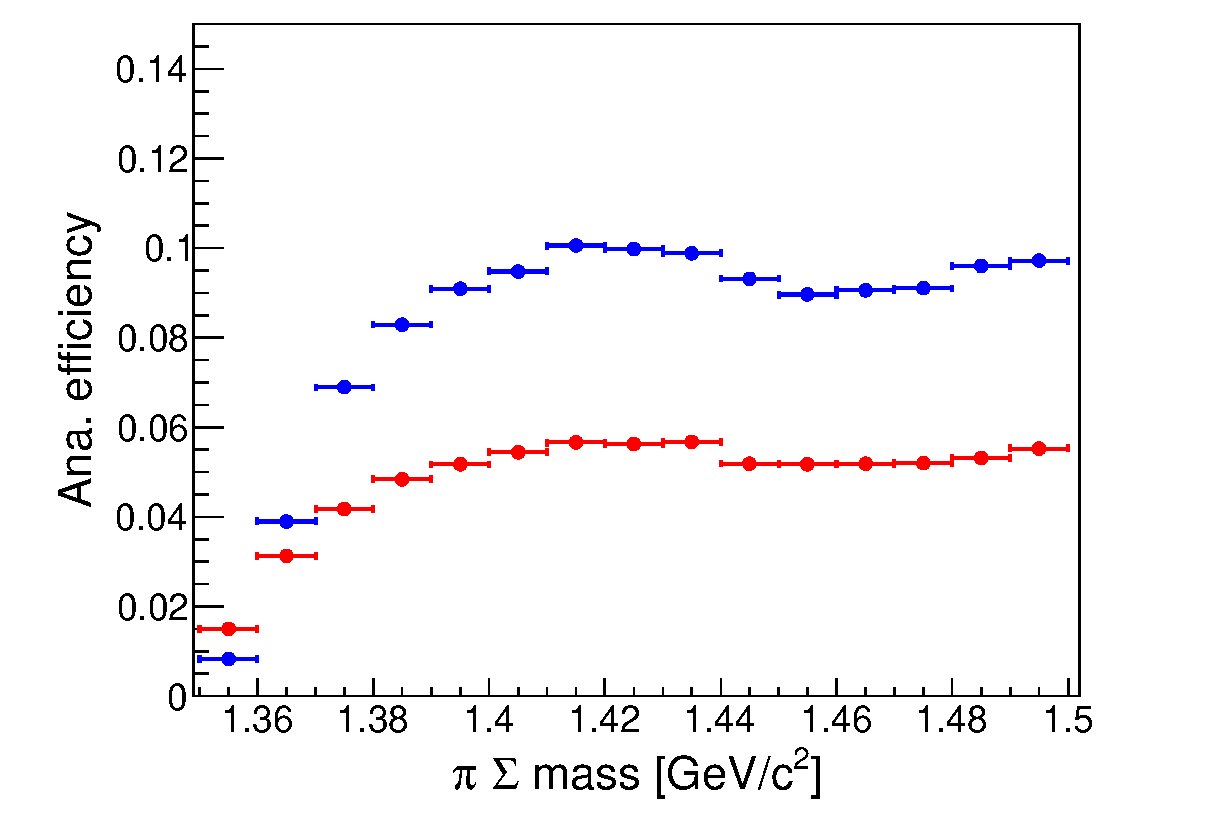
\includegraphics[width=8cm]{../pic/Dron/KN_ana/kn_acc.eps}
  \caption{
    This figure shows the acceptance of $d(K^-, n)"\pi^{\mp}\Sigma^{\pm}"$.
    The red line indicates $\pi^- \Sigma^+$ and the blue line indicates $\pi^+ \Sigma^-$.
  }
  \label{fig:kn_acc}
\end{figure}

\begin{figure}[htbp]
  \centering
  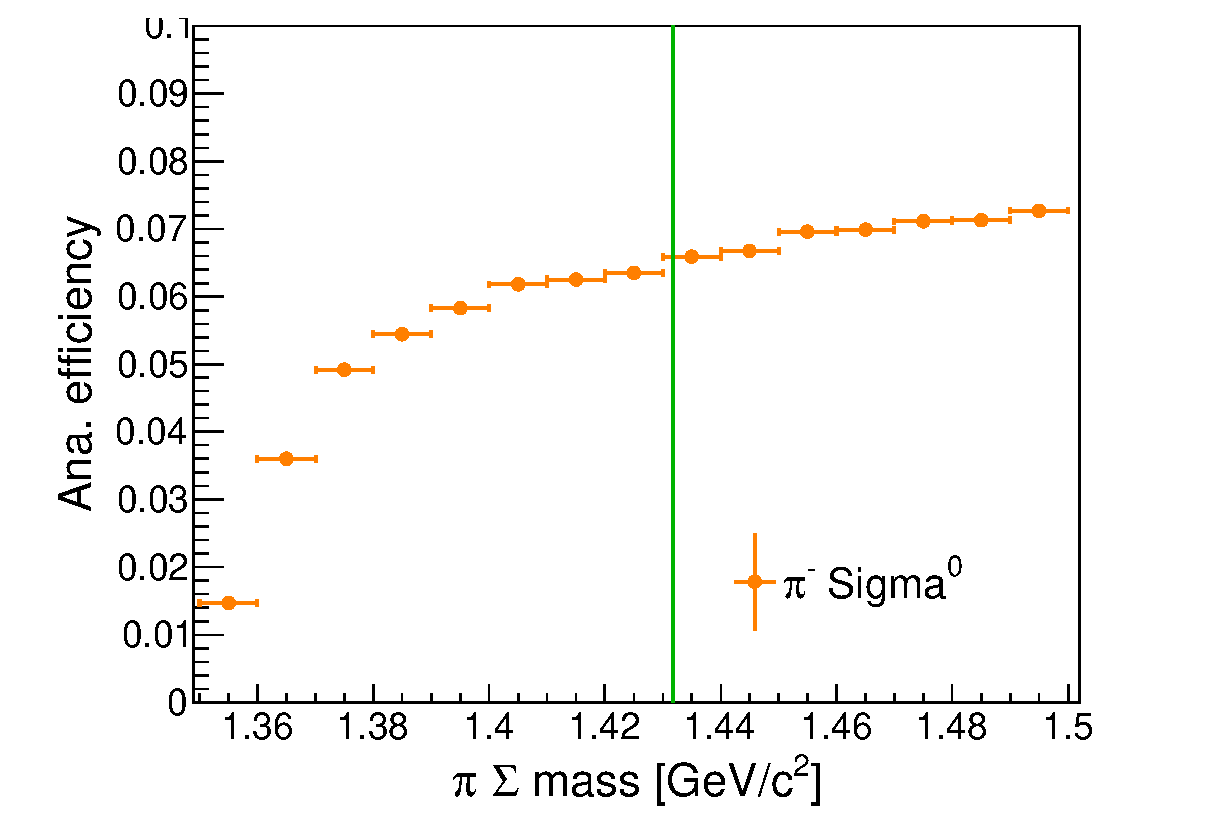
\includegraphics[width=8cm]{../pic/Dron/KP_ana/kp_acc.eps}
  \caption{
    This figure shows $d(K^-, p)"\pi^-\Sigma^0"$ acceptance
  }
  \label{fig:kp_acc}
\end{figure}


This section describes the CDS acceptance correction.
For this correction, we use Monte Carlo simulation data for the $K^-d \rightarrow n \Lambda(1405)$, assuming a 2-step process,
which was also used for the template fitting in the previous section.
The CDS acceptance correction is applied not only to $d(K^-, n)\Lambda(1405)$ but also to $d(K^-, p)\Sigma^*$.
The simulation data for this correction were generated in the same way as for the $K^-d \rightarrow n \Lambda(1405)$ reaction.

The forward-going neutrons (protons) are generated with a slightly wider angular distribution (<8 degrees)
than the acceptance of the forward detector system.
However, since the purpose here is to estimate the CDS acceptance,
only the events that are detected by the forward detector are considered as the sample population.
Among these events, those that pass through the same analysis routine as the real data are regarded as valid events.
In the case of forward neutrons, the analysis includes events in which $\pi^+ \pi^-$ are detected,
followed by the selection of $d(K^-, n \pi^+ \pi^-)n$ events, and the rejection of $K^0$ and $\Sigma^{\pm}_{forward}$.
In the case of forward protons, valid events are those in which $\pi^- \pi^-$ are detected,
and are classified through the $d(K^-, p \pi^- \pi^-)\gamma p$ and $d(K^-, p \pi^-)\Lambda$ selections.

The CDS acceptances obtained for $d(K^-, n)\pi^{\mp}\Sigma^{\pm}$ and $d(K^-, p)\pi^-\Sigma^0$ are shown
in Figures \ref{fig:kn_acc} and \ref{fig:kp_acc}, respectively.



%% The acceptance of $d(K^-,n)"\pi^{\mp}\Sigma^{\pm}"$ and $d(K^-,p)"\pi^-\Sigma^0$ is corrected by MC simulations
%% in which nucleons are injected at a forward angle into the covered region of a forward detector with a uniform $\pi\Sigma$ mass distribution.
%% Since the solid angle of the forward detector is evaluated as subsection.\ref{subsec.XXX}, we adapt as the denominator the events for which the forward detector is analyzable.
%% The same analysis procedure as for the real data is applied to the MC simulation, and the final survival rate is evaluated and used as the acceptance.
%% That is, for $d(K^-, n)"\pi^{\mp}\Sigma^{\pm}"$, we apply $d(K^-, n \pi^+ \pi^-)"n"$ final state selection and rejection of $K^0$ and $\Sigma_{forward}$.
%% For $d(K^-, p)"\pi^-\Sigma^0"$, we apply the $d(K^-, p \pi^- \pi^-)"p \gamma"$ and $d(K^-, p \pi^-)"\Sigma^0"$ selections.
%% Fig.\ref{fig:kn_acc} shows the acceptance of $d(K^-, n)\pi^{\mp} \Sigma^{\pm}$.
%% Dents above the $\bar{K}N$ threshold are due to $K^0$ rejection.
%% The difference in absolute values between $\pi^- \Sigma^+$ and $\pi^+ \Sigma^-$ is due to the branching ratio of the $\Sigma$ decay.
%% Fig.\ref{fig:kp_acc} shows the acceptance of $d(K^-, p)"\pi^-\Sigma^0"$.

%% \begin{frame}{$K^0 cos\theta$ vs mom  {\bf Data}}
  \begin{tabular}{cc}
    \begin{minipage}{0.5\hsize}
      \begin{figure}
        Raw\\
        \includegraphics[width=6cm]{../pic/Run78/QE/K0_cos_mom_data.eps}
      \end{figure}
    \end{minipage}

    \begin{minipage}{0.5\hsize}
      \begin{figure}
        $Data(\cos_{K^0}, p_{K^0}))/A(\cos\theta_{K^0}, p_{K^0})$\\
%%        Accpectance corrected\\
        \includegraphics[width=6cm]{../pic/Run78/QE/K0_cos_mom_data_corr.eps}
      \end{figure}
    \end{minipage}
  \end{tabular}
  
  \centering

  Acceptance was presented at page.4
  
\end{frame}

%% \subsection{The spectrum of the $d(K^-, n)"n K^0"$}

\begin{figure}
  \centering
  \begin{tabular}{cc}
    \begin{minipage}{0.6\hsize}
      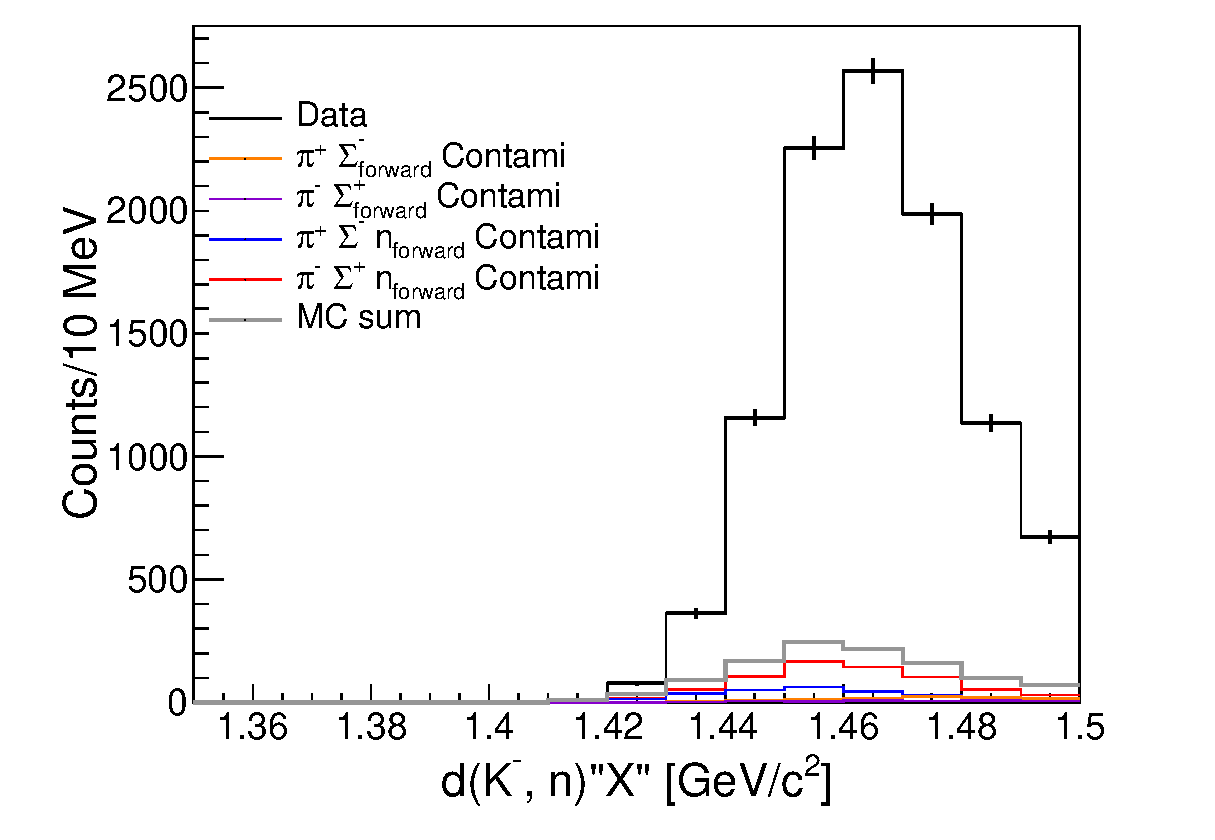
\includegraphics[width=7cm]{../pic/Run78/QE/KN_MM_wK0_tag.eps}
    \end{minipage}
    \begin{minipage}{0.4\hsize}
      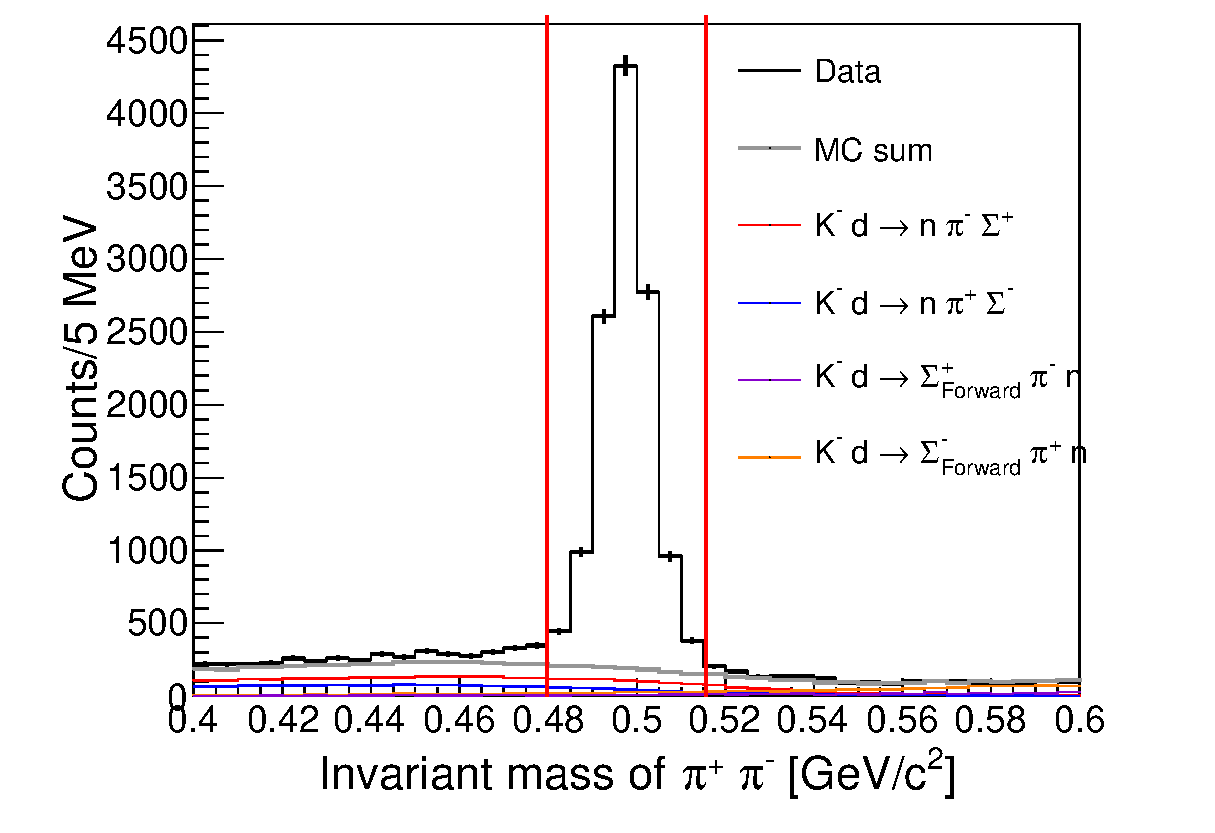
\includegraphics[width=4cm]{../pic/Run78/QE/IM_pipi.eps}
    \end{minipage}
  \end{tabular}
  \caption{
    Right figure shows $K^0$ selection region and estimated background events which is zoom up of left figure of Fig\ref{fig:IM_fit}.
    Red lines indicate selection region.
    left figure shows $d(K^-, n)"n K^0"$ spectra with esmated backgrounds by MC template.
  }
  \label{fig:KN_MM_K0}
\end{figure}

Although the reaction can not measured below the $\bar{K}N$ threshold, 
in the $K^0$ take the strangeness, 
so these events are one of the strongest candidate of the prove for 1-step reaction strength of the $K^-N\rightarrow \bar{K}n$ reaction.\\
The backgrounds were estimated using the template fitting result which was shown in the right figure of Fit\ref{fig:KN_MM_K0}.
The background spectra shape of the $d(K^-, n)"n K^0"$ was indicated in the left figure of the same figure.
These spectra will be collected by the acceptance of the CDS using	the $K^0$ kinematics because detected particles by the CDS came from the $K^0$ decay.
The $K^0$ kinematics was represented as 2 variables function about the $\cos\theta$ and the absolute momentum value and
the acceptance of the CDS was collected event-by-event using the acceptance as weight function as the following equation.

\begin{equation}
  N_{corr}(m_{n K^0}) = \sum N(m_{n K^0}, \cos\theta_{K^0}, p_{K^0}) \cdot \frac{1}{A(\cos\theta_{K^0}, p_{K^0})} \label{eq:corr_K0} 
\end{equation}

\begin{figure}[htbp]
  \centering
  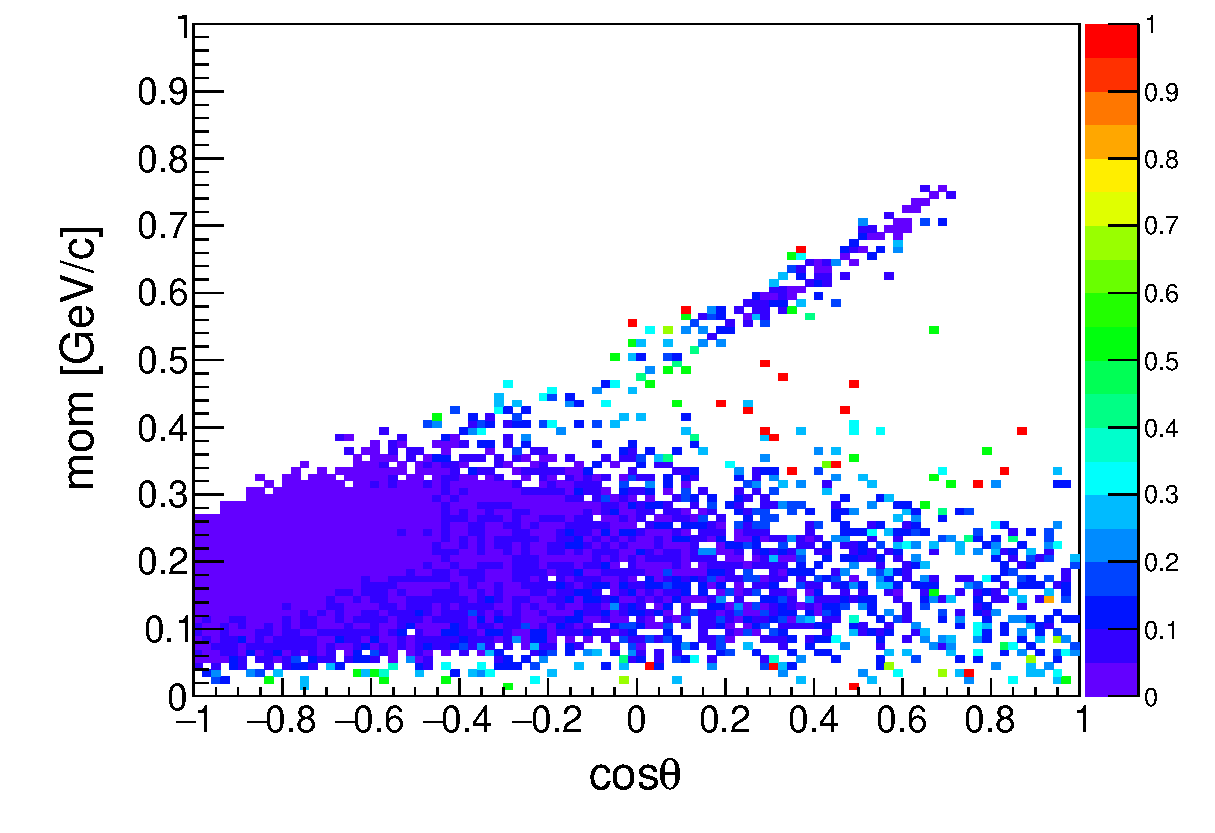
\includegraphics[width=7cm]{../pic/Run78/QE/K0_cos_mom_acc.eps}
  \caption{
    This figure shows the acceptance of the $K^-d\rightarrow K^0 n n$ reaction which was estimated by the Monte Calro simulation.
  }
  \label{fig:K0_acc}
\end{figure}

\begin{figure}[htbp]
  \centering
  \begin{tabular}{cc}
    \begin{minipage}{0.5\hsize}
      \includegraphics[width=7cm]{../pic/Run78/QE/K0_cos_mom_data.eps}
    \end{minipage}

    \begin{minipage}{0.5\hsize}
      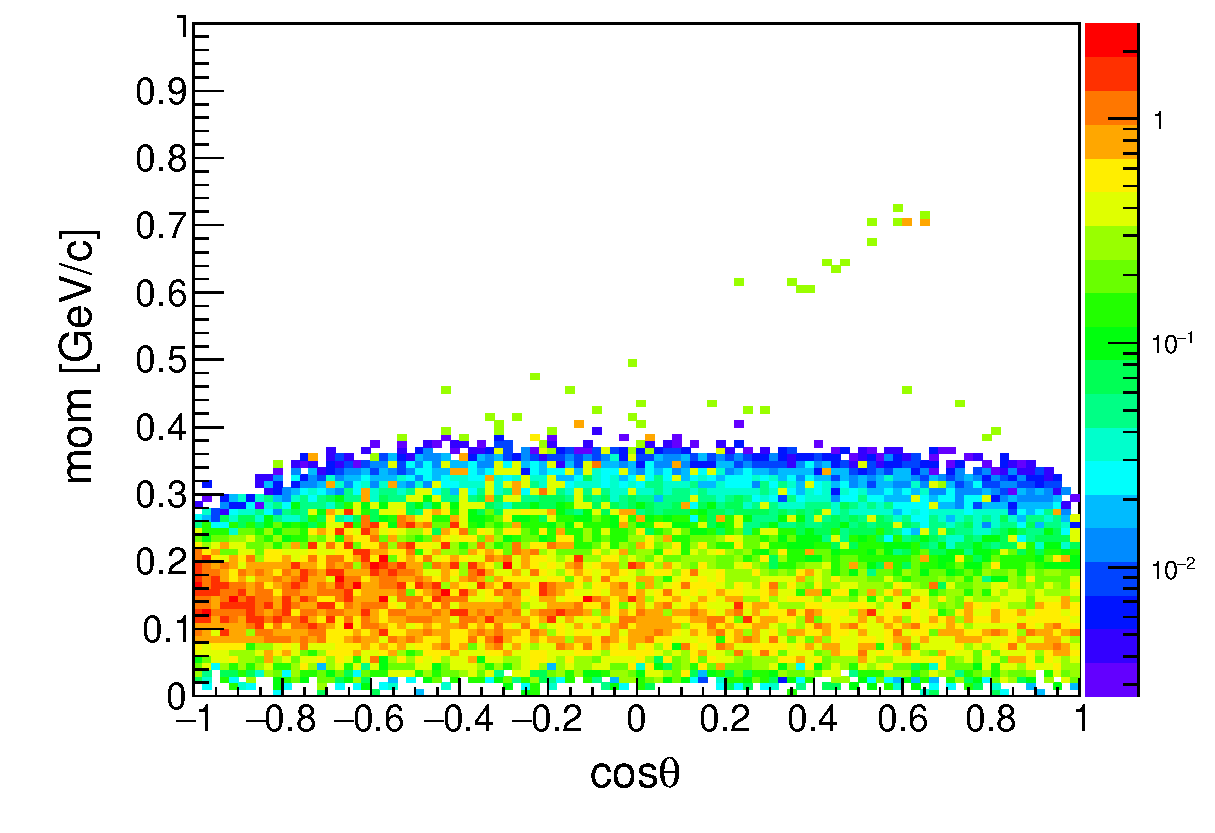
\includegraphics[width=7cm]{../pic/Run78/QE/K0_cos_mom_BG.eps}
    \end{minipage}
  \end{tabular}
  \caption{
    These figure shows about $K^0$ emit angle and momentum in the experimental frame.
    Left figure shows about data and right figure shows background estimated by the Monte Calro.
  }
  \label{fig:K0_cos_mom}
\end{figure}

For this collection, the acceptance was estimated using the $K^- d \rightarrow n_{forwad} (K^0 n)$ reaction.
The mass of the $n K^0$ was generated flat distribution from the $K^0 n$ mass threshold to the kinematical threshold
to accumulate widely and isotropically acceptance which was shown in Fig\ref{fig:K0_acc}
This acceptance collection was adopted to the signal and the backgrounds.
Fig\ref{fig:K0_cos_mom} shows the $K^0$ kinmatics distribution about the data and the backgrounds estimated by the MC sim.
By this operation, we obtained the acceptance collected spectra as shown in Fig\ref{fig:KN_MM_K0_corr}.
Because the data distribution located at the edge of the acceptance and the backgrounds widely distributed, in the acceptance corrected spectra, the signal was enhanced.

\begin{figure}[htbp]
  \centering
  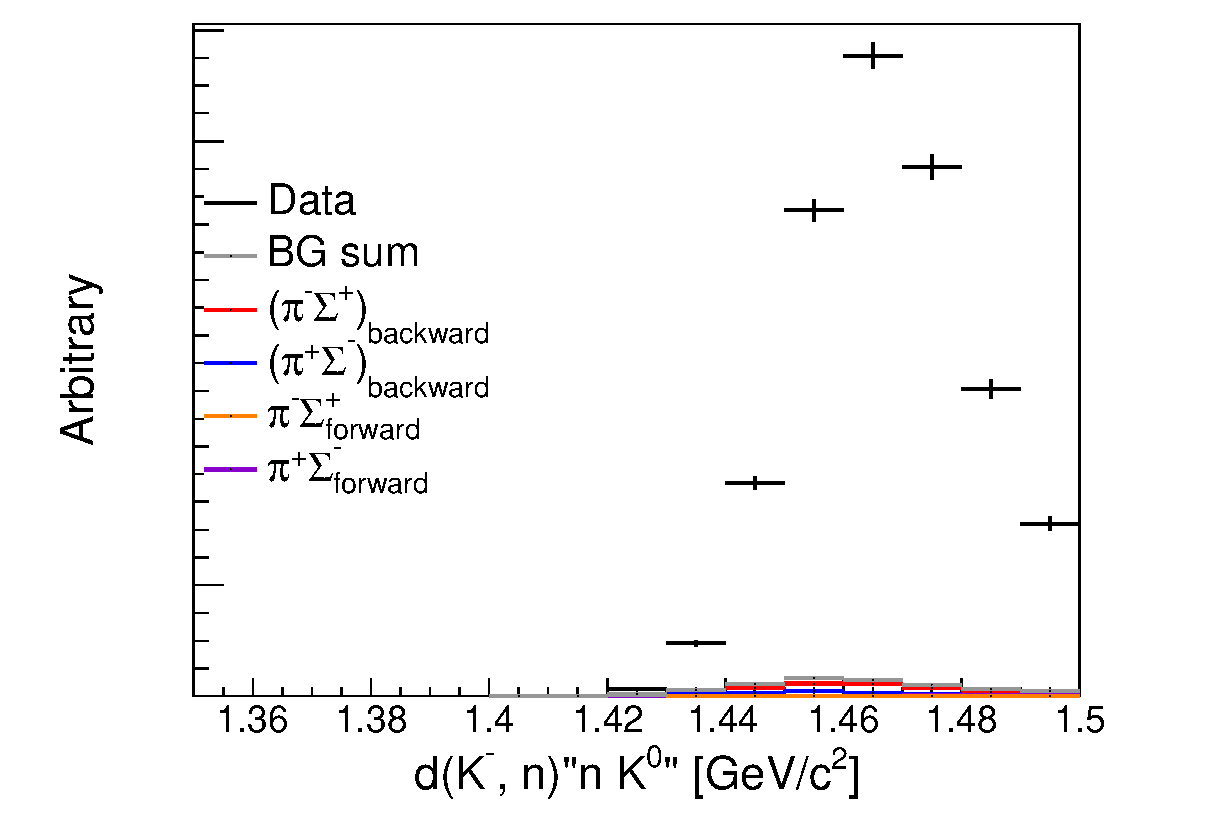
\includegraphics[width=8cm]{../pic/Run78/QE/K0_spec_wBG.eps}
  \caption{
    This figure shows acceptance corrected spectrum of the $d(K^-, n)"n K^0"$.
    Black line indicates data and color plots indicate the background reproduced by the Monte Calro simulation.
  }
  \label{fig:KN_MM_K0_corr}
\end{figure}


%% For $K^0$ production events, we use acceptance for $K^0$ kinematics because all detected particles are of $K^0$ origin.
%% We estimate the two-dimensional acceptances for $K^0$ momentum and $K^0$ scattering angles as shown in Fig\ref{fig.K0_cos_mom_acc}, and weight each event to correct for acceptances.
%% Fig.\ref{fig:K0_spec} shows acceptance corrected spectra of $K^0$ production with reproduced BG by MC simulations.
%% It can be seen that the data are concentrated in the backward and high momentum regions where the acceptances are small,
%% while the MC is distributed over the whole region as shown in Fig.\ref{fig:K0_cos_mom}.
%% In other words, the acceptance correction suppresses BG and emphasizes true $K^0$ production.
